% --------------------------------------------------------------
% This is all preamble stuff that you don't have to worry about.
% Head down to where it says "Start here"
% --------------------------------------------------------------
 
\documentclass[12pt]{article}
 
\usepackage[margin=1in]{geometry} 
\usepackage{amsmath,amsthm,amssymb}
\usepackage{enumerate}

\usepackage{listings}
\usepackage{color}
\usepackage{float}
\usepackage{graphicx}

\definecolor{dkgreen}{rgb}{0,0.6,0}
\definecolor{gray}{rgb}{0.5,0.5,0.5}
\definecolor{mauve}{rgb}{0.58,0,0.82}

\lstset{ %
  language=Octave,                % the language of the code
  basicstyle=\footnotesize,           % the size of the fonts that are used for the code
  numbers=left,                   % where to put the line-numbers
  numberstyle=\tiny\color{gray},  % the style that is used for the line-numbers
  stepnumber=1,                   % the step between two line-numbers. If it's 1, each line 
                                  % will be numbered
  numbersep=5pt,                  % how far the line-numbers are from the code
  backgroundcolor=\color{white},      % choose the background color. You must add \usepackage{color}
  showspaces=false,               % show spaces adding particular underscores
  showstringspaces=false,         % underline spaces within strings
  showtabs=false,                 % show tabs within strings adding particular underscores
  frame=single,                   % adds a frame around the code
  rulecolor=\color{black},        % if not set, the frame-color may be changed on line-breaks within not-black text (e.g. commens (green here))
  tabsize=4,                      % sets default tabsize to 2 spaces
  captionpos=b,                   % sets the caption-position to bottom
  breaklines=true,                % sets automatic line breaking
  breakatwhitespace=false,        % sets if automatic breaks should only happen at whitespace
  title=\lstname,                   % show the filename of files included with \lstinputlisting;
                                  % also try caption instead of title
  keywordstyle=\color{blue},          % keyword style
  commentstyle=\color{dkgreen},       % comment style
  stringstyle=\color{mauve},         % string literal style
  escapeinside={\%*}{*)},            % if you want to add LaTeX within your code
  morekeywords={*,...}               % if you want to add more keywords to the set
}
 
\newcommand{\N}{\mathbb{N}}
\newcommand{\Z}{\mathbb{Z}}
\newcommand{\Q}{\mathbb{Q}}
\newcommand{\R}{\mathbb{R}}
\newcommand{\E}{\mathbb{E}}
\renewcommand{\vec}[1]{\mathbf{#1}}
 
\newenvironment{theorem}[2][Theorem]{\begin{trivlist}
\item[\hskip \labelsep {\bfseries #1}\hskip \labelsep {\bfseries #2.}]}{\end{trivlist}}
\newenvironment{lemma}[2][Lemma]{\begin{trivlist}
\item[\hskip \labelsep {\bfseries #1}\hskip \labelsep {\bfseries #2.}]}{\end{trivlist}}
\newenvironment{exercise}[2][Exercise]{\begin{trivlist}
\item[\hskip \labelsep {\bfseries #1}\hskip \labelsep {\bfseries #2.}]}{\end{trivlist}}
\newenvironment{reflection}[2][Reflection]{\begin{trivlist}
\item[\hskip \labelsep {\bfseries #1}\hskip \labelsep {\bfseries #2.}]}{\end{trivlist}}
\newenvironment{proposition}[2][Proposition]{\begin{trivlist}
\item[\hskip \labelsep {\bfseries #1}\hskip \labelsep {\bfseries #2.}]}{\end{trivlist}}
\newenvironment{corollary}[2][Corollary]{\begin{trivlist}
\item[\hskip \labelsep {\bfseries #1}\hskip \labelsep {\bfseries #2.}]}{\end{trivlist}}
 
\begin{document}
 
% --------------------------------------------------------------
%                         Start here
% --------------------------------------------------------------
 
%\renewcommand{\qedsymbol}{\filledbox}
 
\title{Homework 1}%replace X with the appropriate number
\author{Zhaoheng Zheng\\ %replace with your name
EECS 542 - Machine Learning} %if necessary, replace with your course title
 
\maketitle

\begin{enumerate}[1)]
	\item 
   	\begin {enumerate}[(a)]
    	\item
        \begin{enumerate}[(i)]
       	\item
            \begin{proof} 
                Let symmetric matrix $A \in \mathbb{R}^{2 \times 2}$, 
                  $$A = \left[
                      \begin{matrix}
                          a & b \\
                          b & d
                      \end{matrix}
                  \right]$$

              The inverse of $A$ is,

                  $$A^{-1} = \left[
                      \begin{matrix}
                          \frac{d}{ad-b^{2}} & \frac{-b}{ad-b^{2}} \\
                          \frac{-b}{ad-b^{2}} & \frac{a}{ad-b^{2}}
                      \end{matrix}
                  \right]$$

              Therefore $(A^{-1})^{T} = A^{-1}$, $A^{-1}$ is a symmetric matrix, the statement is \emph{True}.  
          \end{proof}
		\item
            \begin{proof}
                We assume that matrix $A \left[
                        \begin{matrix}
                            a & b \\
                            c & d
                        \end{matrix}
                    \right]$ is orthogonal

               Hence $$ AA^{-1} = AA^{T} = \left[
                        \begin{matrix}
                            a^{2} + b^{2} & ac + bd \\
                            ac + bd & c^{2} + d^{2} \\
                        \end{matrix}
                    \right] = I$$

               Then we have equations
                	\begin{eqnarray*}
                    	a^{2} + b^{2} & = & 1 \\
                        c^{2} + d^{2} & = & 1 \\
                        ac + bd & = & 0
                    \end{eqnarray*}
               We can see that point $(a, b), (c ,d)$ are two points on unit circle. So $\exists \theta, \theta' \in \R$ that satisfy
               		\begin{eqnarray*}
                    	&a = cos\theta , b = sin\theta\\
                        &c = cos\theta' , d = sin\theta'
                    \end{eqnarray*}
               	Hence
                	\begin{align*}
                    	ac + bd & = cos\theta cos\theta' + sin\theta sin\theta'\\
                        & = cos(\theta' - \theta) \\
                        & = 0
                    \end{align*}
                From the equation above we have
                $$ \theta' = \theta + (k + \frac{1}{2})\pi, k\in \Z$$
                When $k$ is even, 
               	$$ A = \left[
                        \begin{matrix}
                            a & b \\
                            c & d
                        \end{matrix}
                    \right]
                    =  \left[
                        \begin{matrix}
                            cos\theta & sin\theta \\
                            cos\theta' & sin\theta'
                        \end{matrix}
                    \right]
                   = \left[
                        \begin{matrix}
                            cos\theta & sin\theta\\
                            -sin\theta & cos\theta
                        \end{matrix}
                    \right]
                   = \left[
                        \begin{matrix}
                            cos(-\theta) & -sin(-\theta)\\
                            sin(-\theta) & cos(-\theta)
                        \end{matrix}
                    \right]$$
               When $k$ is odd,
               $$ A = \left[
                        \begin{matrix}
                            a & b \\
                            c & d
                        \end{matrix}
                    \right]
                    =  \left[
                        \begin{matrix}
                            cos\theta & sin\theta \\
                            cos\theta' & sin\theta'
                        \end{matrix}
                    \right]
                   = \left[
                        \begin{matrix}
                            cos\theta & sin\theta\\
                            sin\theta & -cos\theta
                        \end{matrix}
                    \right]$$
               	Therefore the statement is \emph{True}.
            \end{proof}
        \item
        	\begin{proof}[Disproof]
            	Assume that there exists matrix $C \in \R^{3 \times 3}$ satisfies
                $$A = CC^{T}$$
                Then for any vector $ X \in \R^{3}$,
                \begin{align*}
                	XAX^{T} & = XCC^{T}X^{T} \\
                    		& = (XC)(XC)^T \\
                            & = \langle XC, XC \rangle \geq 0
                \end{align*}
                But if we let
                $$X = \left[
                        \begin{matrix}
                            1 & 0 & 0
                        \end{matrix}
                    \right]$$
                Then
                \begin{align*}
                	XAX^T = -8 < 0
                \end{align*}
                contradicts the inequality $XAX^{T} \geq 0$
                
                Therefore the statement if \emph{False}.
            \end{proof}
\end{enumerate}
\end{enumerate}
	\item
	\begin{enumerate}[(a)]
    	\item
    	\begin{enumerate}[(i)]
			\item
            \begin{proof}
            	\begin{align*}
            		p_{X}(x) & = \int_{y}p(x,y)dy \\
                    & = \int_{y}p_{X|Y}(x|y)p_{Y}(y)dy
                \end{align*}
               	Hence
                \begin{align*}
                	\E[X] & = \int_{x}xp_X(x)dx \\
                    & = \int_{x} x \int_{y} p_{X|Y}(x|y) p_{Y}(y) dy dx \\
                    & = \int_{y} p_{Y}(y) \int_{x} x p_{X|Y}(x|y) dx dy \\
                    & = \int_{y} p_{Y}(y) \E_{X}[X|Y] dy \\
                    & = \E_{Y}[\E_{X}[X|Y]]
                \end{align*}
            \end{proof}
           	\item
            \begin{proof}
            	\begin{align*}
            		\E[I[X \in \mathcal{C}]] & = \int_{x} I[x \in \mathcal{C}]p_{X}(x) dx \\
                	& = \int_{x \in \mathcal{C}} p_{X}(x) dx \\
                	& = P(X \in \mathcal{C})
                \end{align*}
            \end{proof}
            \item 
            \begin{proof}
            	We first prove $var[X] = \E[X^{2}] - (\E[X])^{2}$:
                \begin{align*}
                	\text{var}[X] & = \int_{x} (x - \E[X])^{2} p_{X}(x) dx \\
                    & = \int_{x} (x^{2} - 2x\E[X] + [\E[X]]^{2}) p_{X}(x)dx \\
                    & = \E(X^{2}) - 2(\E[X])^{2} + (\E[X])^{2} \\
                    & = \E(X^{2}) - (\E[X])^{2}
                \end{align*}
                Hence, we obtain   
                $$ \E_{Y}[\text{var}_{X}[X | Y]] = \E_{Y}[\E_{X}[X^{2} | Y]] - \E_{Y}[(\E_{X}[X|Y])^{2}]] = \E[X^{2}] - \E_{Y}[(\E_{X}[X|Y])^{2}]$$           
                $$ \text{var}_{Y}[\E_{X}[X|Y]] = \E_{Y}[\E_{X}[X|Y]^{2}] - \E_{Y}[\E_{X}[X|Y]]^{2} = \E_{Y}[(\E_{X}[X|Y])^{2}] - (\E[X])^{2}$$
                
                Therefore $\E_{Y}[\text{var}_{X}[X | Y]] + \text{var}_{Y}[\E_{X}[X|Y]] = \E[X^{2}] - (\E[X])^{2} = \text{var}[X]$.
            \end{proof}
           	\item
            \begin{proof}
            	Since $X$ and $Y$ are independent, we obtain $p(x, y) = p_{x}(x)p_{y}(y)$. Therefore, 
                \begin{align*}
                	\E[XY] & = \int_{x}\int_{y}xyp(x,y)dydx \\
                    & = \int_{x} \int_{y} xp_{X}(x)yp_{Y}(y)dydx \\
                    & = \int_{x} xp_{X}(x) \bigg[ \int_{y} yp_{Y}(y)dy \bigg] dx \\
                    & = \E[Y] \int_{x} xp_{X}(x)dx \\
                    & = \E[X]\E[Y]
                \end{align*}
            \end{proof}
            \item
            \begin{proof}
            	Since $X$ and $Y$ takes value in $\{0, 1\}$, we obtain
                $$\E[X] = P(X = 1), \quad \E[Y] = P(Y = 1)$$
                Then we can get
                $$\E[XY] = P(X = 1, Y = 1) = \E[X]\E[Y] = P(X = 1) P(Y = 1)$$
                Hence
                \begin{eqnarray*}
                	&P(X=1, Y=0) = P(X=1) - P(X=1,Y=1) = P(X=1)P(Y=0) \\
                    &P(X=0, Y=1) = P(Y=1) - P(X=1,Y=1) = P(X=0)P(Y=1) \\
                    &P(X=0, Y=0) = P(X=0) - P(X=0,Y=1) = P(X=0)P(Y=0) 
                \end{eqnarray*}
               	Therefore $P(X, Y) = P(X)P(Y), X,Y$ are independent.
            \end{proof}
        \end{enumerate}
        \item
        \begin{enumerate}[(i)]
        	\item $P(H=h, D=d) \leq P(H=h)$
            
           	\begin{proof} We can obtain that
            	$$P(H=h) = \sum_{d}P(H=h,D=d)$$
                For any $d, P(H=h, D=d) \geq 0$,
                
                Therefore $P(H=h) = \sum_{d}P(H=h,D=d) \geq P(H=h,D=d)$.
            \end{proof}
            \item It depends. 
            
            Since $P(H=h|D=d) = \frac{P(H=h, D=d)}{P(D=d)}$ and we can't decide the value of $P(D=d) \in (0, 1) $, it depends.
           	\item       		$P(H=h|D=d) \geq P(D=d|H=h)P(H=h)$,
                    \begin{proof}
            $$ P(H=h|D=d) = \frac{P(H=h, D=d)}{P(D=d)} $$
            Therefore $$ P(D=d|H=h)P(H=h) = P(H=h, D=d) \leq P(H=h|D=d)$$
  			\end{proof}
        \end{enumerate}
    \end{enumerate}
    \item
    \begin{enumerate}[(a)]
    	\item 
        \begin{proof}        	Since $U^{T}U = UU^{T} = I$, we can obtain that for any column vector $\mathbf{u}_{i}$. So$$\vec{u}_{i}^{T}\vec{u}_{i} = 1$$
            
            We first assume that matrix $A$ is PSD, then for each eigenvalue $\lambda_{i}$ , we obtain
            $$\vec{u}_{i}^{T}A\vec{u}_{i} = \vec{u}_{i}^{T}\lambda_{i}\vec{u}_{i} = \lambda_{i}\vec{u}_{i}^{T}\vec{u}_{i}  = \lambda_{i} \geq 0$$
                   
            Then we assume for each $i$, $\lambda_{i} \geq 0$. For all $\vec{x} \in \R^{d}$,
            \begin{align*}
           \vec{x}^{T}A\vec{x} & = \vec{x}^{T}U\Lambda U^{T} \vec{x}\\
           & = \vec{x}^{T}\sum_{i=1}^{d}\lambda_{i}\vec{u}_{i}\vec{u}_{i}^{T}\vec{x} \\
           &=  \sum_{i=1}^{d}\lambda_{i}(\vec{x}^{T}\vec{u}_{i})(\vec{x}^{T}\vec{u}_{i})^{T} \\
           & = \sum_{i=1}^{d}\lambda_{i}(\vec{x}^{T}\vec{u}_{i})^{2}
           \end{align*}
           Since for each $i, \lambda_{i} \geq 0$.  Hence for each $\vec{x} \in \R^{d}$
           $$\vec{x}^{T}A\vec{x}  = \sum_{i=1}^{d}\lambda_{i}(\vec{x}^{T}\vec{u}_{i})^{2}\geq 0$$
           Therefore $A$ is PSD iff $\lambda_{i} \geq 0$ for each $i$.
        \end{proof}
        \item
        \begin{proof}
        	We first assume that matrix $A$ is PD, then for each eigenvalue $\lambda_{i}$ , we obtain
            $$\vec{u}_{i}^{T}A\vec{u}_{i} = \vec{u}_{i}^{T}\lambda_{i}\vec{u}_{i} = \lambda_{i}\vec{u}_{i}^{T}\vec{u}_{i}  = \lambda_{i} > 0$$
             
            Then we assume for each $i$, $\lambda_{i} > 0$. For all $\vec{x} \in \R^{d}$,
            \begin{align*}
           \vec{x}^{T}A\vec{x} & = \vec{x}^{T}U\Lambda U^{T} \vec{x}\\
           & = \vec{x}^{T}\sum_{i=1}^{d}\lambda_{i}\vec{u}_{i}\vec{u}_{i}^{T}\vec{x} \\
           &=  \sum_{i=1}^{d}\lambda_{i}(\vec{x}^{T}\vec{u}_{i})(\vec{x}^{T}\vec{u}_{i})^{T} \\
           & = \sum_{i=1}^{d}\lambda_{i}(\vec{x}^{T}\vec{u}_{i})^{2}
           \end{align*}
           Now we prove that there is no $\vec{x} \neq \vec{0}, \vec{x}^{T}\vec{u}_{i}  = 0$ for each $i$.
           
           Assume that for each $i$, we have $\vec{x} \neq \vec{0}$ that $\vec{x}^{T}\vec{u}_{i} = 0$, we can let matrix $X \in \R^{d}$ be
           $$X = \left[
           	\begin{matrix}
            		\vec{x}   \cdots  \vec{x}
            \end{matrix}
           \right]$$
           Then 
           $$ X^{T}UU^{T} = \left[
           \begin{matrix}
           		\vec{x}^{T} \\
                \vdots \\
                \vec{x}^{T}
           \end{matrix}
           \right]
           \left[
           \begin{matrix}
           		\vec{u}_{1}  \vec{u}_{2} \cdots \vec{u}_{d}
           \end{matrix}
           \right] U^{T} = \vec{0} \cdot U^{T} = \vec{0}$$
			However,
            $$  X^{T}UU^{T} = X^{T}I = X^{T} \neq \vec{0} $$
            which contradicts the equation above. Hence there is no $\vec{x} \neq \vec{0}, \vec{x}^{T}\vec{u}_{i}  = 0$ for each $i$.
            
            Therefore
                       $$\vec{x}^{T}A\vec{x}  = \sum_{i=1}^{d}\lambda_{i}(\vec{x}^{T}\vec{u}_{i})^{2} > 0$$
              implies $A$ is PD.
        \end{proof}
    \end{enumerate}
    \item
    \begin{enumerate}[(a)]
    	\item
        \begin{proof}
        \begin{align*}
        	f(t\vec{x}+(1-t)\vec{y}) & = \vec{a}^{T}(t\vec{x} + (1-t)\vec{y}) + b \\
            & = t(\vec{a}^{T}x + b) + (1-t)(\vec{a}^{T}y + b) \\
            & = tf(\vec{x}) + (1-t)f(\vec{y})
        \end{align*}
        \end{proof}
        So affine function $f(\vec{x}) = \vec{a}^{T}\vec{x} + b$ is convex.
        And 
        \begin{align*}
        	-f(t\vec{x} + (1-t)\vec{y}) & = -( \vec{a}^{T}(t\vec{x} + (1-t)\vec{y}) + b) \\
            & = -t(\vec{a}^{T}x + b) - (1-t)(\vec{a}^{T}y + b) \\
            & = t(-f(\vec{x})) + (1-t)(-f(\vec{y}))
        \end{align*}
        Therefore $f(\vec{x})$ is convex and concave.
        
        Since for all $\vec{x}, \vec{y}$ in the domain of $f$, $$f(t\vec{x} + (1-t)\vec{y})= tf(\vec{x}) + (1-t)f(\vec{y})$$  $f(\vec{x})$ is not strictly convex.
        \item
        \begin{proof}
        	Assume that $f$ has more than one global minimizers,  we denote two of them as $\vec{x}_{1}, \vec{x}_{2}$.
            
            For any $t \in [0, 1]$, we let $\vec{x}_{t} = t\vec{x}_{1} + (1-t)\vec{x}_{2}$. Since $f$ is strictly convex, we can obtain that inequality:
            $$f(\vec{x}_{t}) = f(t\vec{x}_{1} + (1-t)\vec{x}_{2}) < tf(\vec{x}_{1}) + (1-t)f(\vec{x}_{2}) = f(\vec{x}_{1}) = f(\vec{x}_{2})$$
            which contradicts the statement that $\vec{x}_{1}, \vec{x}_{2}$ are global minimizers.
            
            Therefore, if $f$ is strictly convex, then $f$ has at most one global minimizer.
        \end{proof}
        \item
        \begin{proof}
        	Since $\vec{x}^{*}$ is a local minimizer,  we can obtain
            $$\nabla f(\vec{x}^{*}) = 0$$
            For all $\vec{x}$ in the neighborhood of $\vec{x}^{*}$,
            \begin{align*}
            	f(\vec{x}) - f(\vec{x}^{*}) & = \langle \nabla f(\vec{x}^{*}), \vec{x} - \vec{x}^{*} \rangle + \frac{1}{2} \langle \vec{x} - \vec{x}^{*}, \nabla^{2}f(\vec{x}^{*})(\vec{x} -\vec{x}^{*})\rangle + o(||\vec{x} - \vec{x}^{*}||^{2}) \\
                & = \frac{1}{2} \langle \vec{x} - \vec{x}^{*}, \nabla^{2}f(\vec{x}^{*})(\vec{x} -\vec{x}^{*})\rangle + o(||\vec{x} - \vec{x}^{*}||^{2}) \geq 0
            \end{align*}
           Then
           \begin{align*}
           	\lim_{\vec{x} \rightarrow \vec{x}^{*}} \frac{f(\vec{x}) - f(\vec{x}^{*})}{||\vec{x} - \vec{x}^{*}||^{2}}  & = \lim_{\vec{x} - \vec{x}^{*}}\bigg[\frac{1}{2} \frac{\langle \vec{x} - \vec{x}^{*}, \nabla^{2}f(\vec{x}^{*})(\vec{x} -\vec{x}^{*})\rangle}{||\vec{x} - \vec{x}^{*}||^{2}} + \frac{o(||\vec{x} - \vec{x}^{*}||^{2})}{||\vec{x} - \vec{x}^{*}||^{2}}\bigg] \\
            & = \lim_{\vec{x} - \vec{x}^{*}}\bigg[\frac{1}{2} \frac{\langle \vec{x} - \vec{x}^{*}, \nabla^{2}f(\vec{x}^{*})(\vec{x} -\vec{x}^{*})\rangle}{||\vec{x} - \vec{x}^{*}||^{2}}\bigg] \geq 0
           \end{align*}
           Hence $\langle \vec{x} - \vec{x}^{*}, \nabla^{2}f(\vec{x}^{*})(\vec{x} -\vec{x}^{*})\rangle \geq 0$. 
           
           So for all direction $\vec{h}$, $$\langle \vec{h}, \nabla^{2}f(\vec{x}^{*}){h} \rangle \geq 0$$ 
           Therefore $\nabla^{2}f(\vec{x}^{*})$ is positive semi-definite.
        \end{proof}
        \item
        \begin{proof}
        	We first assume that $\nabla^{2} f(\vec{x})$ is positive semi-definite for all $\vec{x} \in \R^{d}$.
            Denote $g(t) = f(t\vec{x}  + (1-y)\vec{y})$, we can obtain
            $$g'(t) = (\vec{x} - \vec{y})^{T}\nabla f(t\vec{x} + (1-t)\vec{y})$$
            $$g''(t) = (\vec{x} - \vec{y})^{T}\nabla^{2}f(t\vec{x} + (1-t)\vec{y})(\vec{x} - \vec{y})$$
            Since $\nabla^{2} f(\vec{x})$ is positive semi-definite for all $\vec{x} \in \R^{d}$, we can get that for all $t$, $g''(t) \geq 0$.
            
            Then according to Taylor series, we obtain
            $$ g(0) = g(t) + g'(t)(-t) + \frac{1}{2}g''(t-\theta t)t^{2} \geq g(t) + g'(t)(-t)$$
            $$g(1) = g(t) + g'(t)(1-t) + \frac{1}{2}g''(t + \theta(1-t))(1-t)^{2} \geq g(t) + g'(t)(1-t)$$
        	Thus for $t \in [0, 1]$,
            $$ (1-t)g(0) + tg(1) \geq (1-t)g(t) + g'(t)(1-t)(-t) + tg(t) + g'(t)(1-t)t = g(t) $$
            which implies 
            $$f(t\vec{x} + (1-t)\vec{y}) \leq tf(\vec{x}) + (1-t)f(\vec{y})$$
            Hence $f(\vec{x})$ is convex.
            
            Now we assume $f(\vec{x})$ is convex, by definition, for any $t \in [0, 1]$
            $$f(t\vec{x} + (1-t)\vec{y}) \leq tf(\vec{x}) +  (1-t)f(\vec{y})$$
            We can rewrite the inequality into
            $$f(t\vec{x} + (1-t)\vec{y}) \leq t[f(\vec{x}) - f(\vec{y})] +  f(\vec{y})$$
			Then for any $t \in (0, 1]$, 
            $$f(\vec{x}) - f(\vec{y}) \geq \frac{f(t\vec{x} + (1-t)\vec{y}) - f(\vec{y})}{t}$$
            When $t \rightarrow 0$, we get
            $$f(\vec{x}) - f(\vec{y}) \geq \langle \nabla f(\vec{y}),  \vec{x} - \vec{y} \rangle$$
            implies 
            $$\frac{1}{2}\frac{\langle \vec{x} - \vec{y}, \nabla^{2}f(\vec{y})(\vec{x} - \vec{y}) \rangle}{||\vec{x} - \vec{y}||^{2}} + \frac{o(||\vec{x} - \vec{y}||^{2})}{||\vec{x} - \vec{y}||^{2}} $$
            Limit $\vec{x} \rightarrow \vec{y}$, $\langle \vec{x} - \vec{y}, \nabla^{2}f(\vec{y})(\vec{x} - \vec{y}) \rangle \geq 0$ for all $\vec{y} \in \R^{d}$.
            
            Therefore, $\nabla^{2} f(\vec{x})$ is positive semi-definite for all $\vec{x} \in \R^{d}$
            \end{proof}
            \item
            \begin{proof}[Solution]
            	The first derivative $\nabla f(\vec{x})$ is $A\vec{x} + \vec{b}$, while the Hessian is $A$. 
                
                When $A$ is a positive semi-definite matrix, $f$ is convex.
                
                When $A$ is positive definite, $f$ is strictly convex.
            \end{proof}
    \end{enumerate}
    \item 
    \begin{enumerate}[(a)]
    	\item The result and ratio for $k$-approximation are shown below:
        \begin{enumerate}[(i)]
        	\item $k = 2, \frac{||X - \tilde{X}||_{F}}{||X||_{F}}=0.281484$,
   \begin{figure}[H] % use float package if you want it here
  \centering
  
\includegraphics[width=0.5\textwidth]{2_app}
  \caption{Approximation image for $k$=2}
\end{figure}

        	\item $k = 10, \frac{||X - \tilde{X}||_{F}}{||X||_{F}}=0.158739$,
   \begin{figure}[H] % use float package if you want it here
  \centering
  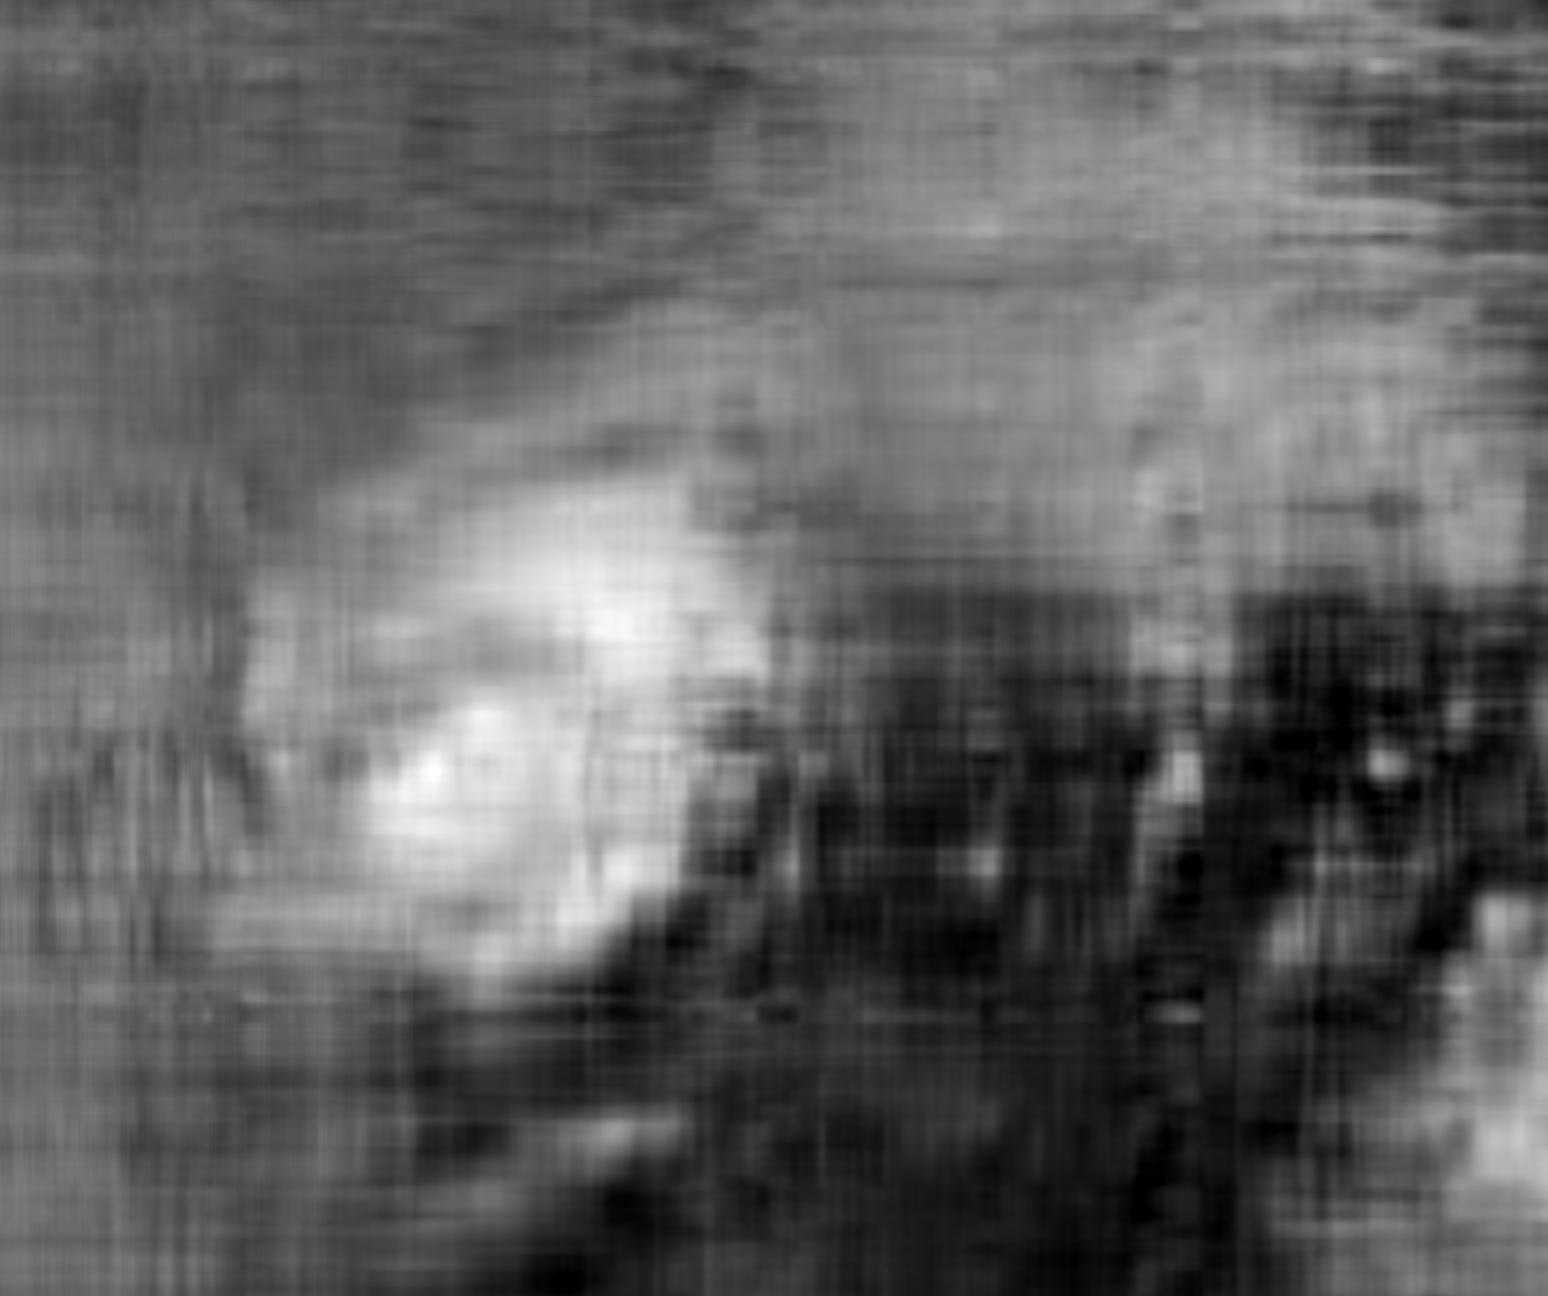
\includegraphics[width=0.5\textwidth]{10_app}
  \caption{Approximation image for $k$=10}
\end{figure}

        	\item $k = 40, \frac{||X - \tilde{X}||_{F}}{||X||_{F}}=0.083671$,
   \begin{figure}[H] % use float package if you want it here
  \centering
  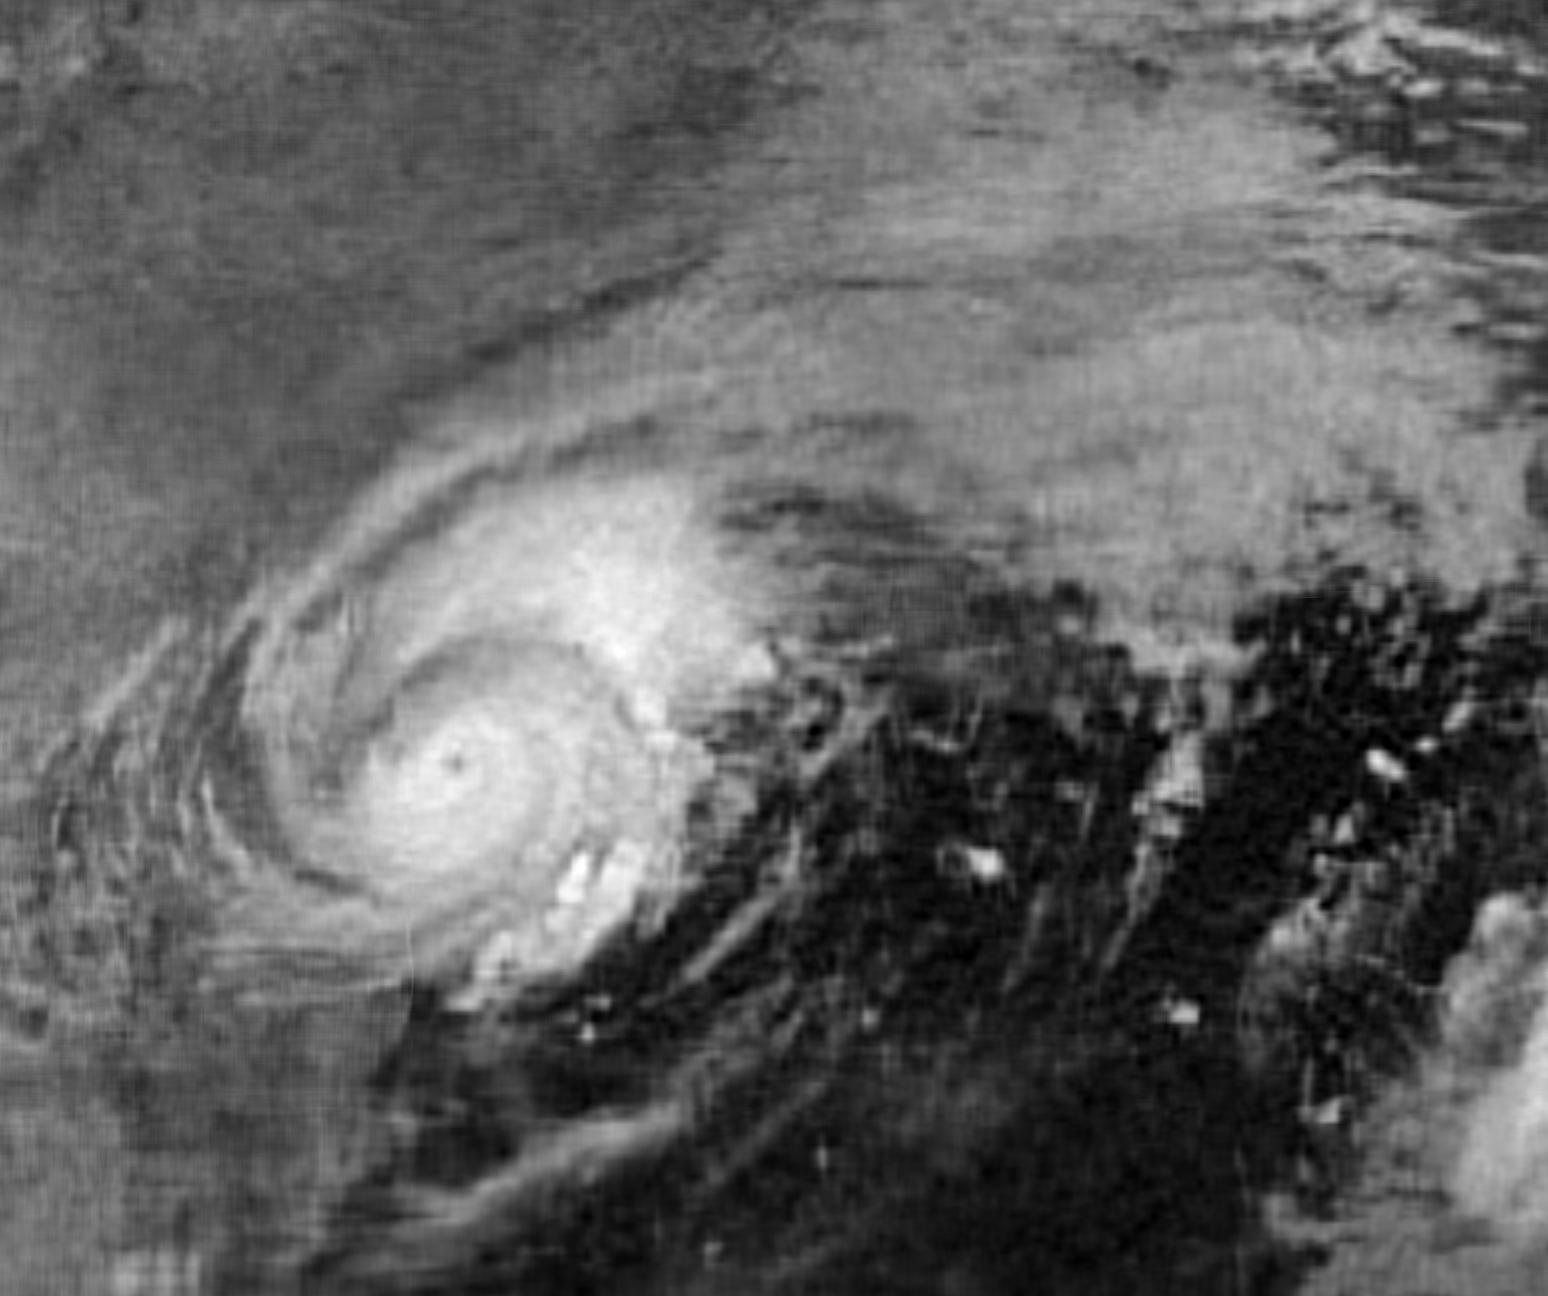
\includegraphics[width=0.5\textwidth]{40_app}
  \caption{Approximation image for $k$=40}
\end{figure}
        \end{enumerate}
        \item The numbers to describe the approximation $\tilde{X}_{k}$ for $k=\{2, 10,  40\}$ are$\{5690, 28450, 113800\}$
        \item The code are shown below:
        \begin{lstlisting}
X = double(rgb2gray(imread('harvey-saturday-goes7am.jpg')));
[U, S, V] = svd(X);

k = [2 10 40];

for i=1:3
    app_x = zeros(size(X));
    sum_num = 0;
    for j = 1:k(i)
        app_x = app_x + S(j, j) * U(:, j) * V(:, j)';
        sum_num = sum_num + 1 + size(U(:, j)) + size(V(:, j));
    end
    s = sprintf('%d_app.jpg', k(i));
    imwrite(app_x / 256, s);
    ratio = norm(X - app_x, 'fro') / norm(X, 'fro');
    fprintf('Top %d approximation, error: %f\n', k(i), ratio);
    fprintf('numbers to store: %d\n', sum_num(1));
end
        \end{lstlisting}
    \end{enumerate}
\end{enumerate}


% --------------------------------------------------------------
%     You don't have to mess with anything below this line.
% --------------------------------------------------------------
 
\end{document}